\documentclass[man]{apa6}
\usepackage{lmodern}
\usepackage{amssymb,amsmath}
\usepackage{ifxetex,ifluatex}
\usepackage{fixltx2e} % provides \textsubscript
\ifnum 0\ifxetex 1\fi\ifluatex 1\fi=0 % if pdftex
  \usepackage[T1]{fontenc}
  \usepackage[utf8]{inputenc}
\else % if luatex or xelatex
  \ifxetex
    \usepackage{mathspec}
  \else
    \usepackage{fontspec}
  \fi
  \defaultfontfeatures{Ligatures=TeX,Scale=MatchLowercase}
\fi
% use upquote if available, for straight quotes in verbatim environments
\IfFileExists{upquote.sty}{\usepackage{upquote}}{}
% use microtype if available
\IfFileExists{microtype.sty}{%
\usepackage{microtype}
\UseMicrotypeSet[protrusion]{basicmath} % disable protrusion for tt fonts
}{}
\usepackage{hyperref}
\hypersetup{unicode=true,
            pdftitle={Domain-specific working memory loads selectively increase negative interpertations of surprised facial expressions},
            pdfauthor={Nicholas R. Harp~\& Maital Neta},
            pdfkeywords={ambiguity, working memory, bias},
            pdfborder={0 0 0},
            breaklinks=true}
\urlstyle{same}  % don't use monospace font for urls
\usepackage{graphicx,grffile}
\makeatletter
\def\maxwidth{\ifdim\Gin@nat@width>\linewidth\linewidth\else\Gin@nat@width\fi}
\def\maxheight{\ifdim\Gin@nat@height>\textheight\textheight\else\Gin@nat@height\fi}
\makeatother
% Scale images if necessary, so that they will not overflow the page
% margins by default, and it is still possible to overwrite the defaults
% using explicit options in \includegraphics[width, height, ...]{}
\setkeys{Gin}{width=\maxwidth,height=\maxheight,keepaspectratio}
\IfFileExists{parskip.sty}{%
\usepackage{parskip}
}{% else
\setlength{\parindent}{0pt}
\setlength{\parskip}{6pt plus 2pt minus 1pt}
}
\setlength{\emergencystretch}{3em}  % prevent overfull lines
\providecommand{\tightlist}{%
  \setlength{\itemsep}{0pt}\setlength{\parskip}{0pt}}
\setcounter{secnumdepth}{0}
% Redefines (sub)paragraphs to behave more like sections
\ifx\paragraph\undefined\else
\let\oldparagraph\paragraph
\renewcommand{\paragraph}[1]{\oldparagraph{#1}\mbox{}}
\fi
\ifx\subparagraph\undefined\else
\let\oldsubparagraph\subparagraph
\renewcommand{\subparagraph}[1]{\oldsubparagraph{#1}\mbox{}}
\fi

%%% Use protect on footnotes to avoid problems with footnotes in titles
\let\rmarkdownfootnote\footnote%
\def\footnote{\protect\rmarkdownfootnote}


  \title{Domain-specific working memory loads selectively increase negative interpertations of surprised facial expressions}
    \author{Nicholas R. Harp\textsuperscript{1}~\& Maital Neta\textsuperscript{1}}
    \date{}
  
\shorttitle{DOMAIN-SPECIFIC WORKING MEMORY AND SURPRISED EXPRESSIONS}
\affiliation{
\vspace{0.5cm}
\textsuperscript{1} University of Nebraska-Lincoln}
\keywords{ambiguity, working memory, bias\newline\indent Word count: X}
\usepackage{csquotes}
\usepackage{upgreek}
\captionsetup{font=singlespacing,justification=justified}

\usepackage{longtable}
\usepackage{lscape}
\usepackage{multirow}
\usepackage{tabularx}
\usepackage[flushleft]{threeparttable}
\usepackage{threeparttablex}

\newenvironment{lltable}{\begin{landscape}\begin{center}\begin{ThreePartTable}}{\end{ThreePartTable}\end{center}\end{landscape}}

\makeatletter
\newcommand\LastLTentrywidth{1em}
\newlength\longtablewidth
\setlength{\longtablewidth}{1in}
\newcommand{\getlongtablewidth}{\begingroup \ifcsname LT@\roman{LT@tables}\endcsname \global\longtablewidth=0pt \renewcommand{\LT@entry}[2]{\global\advance\longtablewidth by ##2\relax\gdef\LastLTentrywidth{##2}}\@nameuse{LT@\roman{LT@tables}} \fi \endgroup}


\DeclareDelayedFloatFlavor{ThreePartTable}{table}
\DeclareDelayedFloatFlavor{lltable}{table}
\DeclareDelayedFloatFlavor*{longtable}{table}
\makeatletter
\renewcommand{\efloat@iwrite}[1]{\immediate\expandafter\protected@write\csname efloat@post#1\endcsname{}}
\makeatother
\usepackage{lineno}

\linenumbers

\authornote{Nicholas R. Harp, Department of Psychology, Center for Brain, Biology, and Behavior, University of Nebraska-Lincoln
Maital Neta, Department of Psychology, Center for Brain, Biology, and Behavior, University of Nebraska-Lincoln

Correspondence concerning this article should be addressed to Nicholas R. Harp, Postal address. E-mail: \href{mailto:nharp@huskers.unl.edu}{\nolinkurl{nharp@huskers.unl.edu}}}

\abstract{
Individual differences in interpretations of emotional ambiguity are a useful tool for measuring affective biases.

While trait-like, these biases are also susceptible to experimental manipulations. In the present study, we capitalize on this malleability to expand on previous research suggesting that
subjective interpretations are stable independently of cognitive load.

We tested the effects of working memory loads containing either neutral or emotional content on concurrent interpretations of surprised facial expressions.

Here we show that interpretations of surprise are more negative during maintenance of working memory loads with emotional content compared to those with neutral content.

Two or three sentences explaining what the \textbf{main result} reveals in direct comparison to what was thought to be the case previously, or how the main result adds to previous knowledge.

One or two sentences to put the results into a more \textbf{general context}.

Two or three sentences to provide a \textbf{broader perspective}, readily comprehensible to a scientist in any discipline.


}

\begin{document}
\maketitle

\hypertarget{introduction}{%
\section{Introduction}\label{introduction}}

\hypertarget{working-memory-and-load-theory}{%
\subsection{Working memory and load theory}\label{working-memory-and-load-theory}}

Despite extensive research on the interaction of working memory and affective processes, there is much to learn concerning how cognitive and emotional processes affect one another. Executive functions, including working memory, are related to successful self-regulation, and in turn emotion regulation (Hofmann, Schmeichel, \& Baddeley, 2012). Directly comparing working memory and self-regulation of emotional responses, Schmeichel and colleagues (2008) reported that individuals with higher levels of working memory capacity demonstrated improved self-regulation towards the emotional stimuli. This suggests a connection--perhaps through some shared resource pool--between mitigated emotional responding and larger working memory resource availablility. Other work has focused on the effects of moods or affective states on working memory performance. For instance, some reports claim that both positive and negative mood interfere with working memory (Eyesenck and Calvo, 1992); however, others suggest benefits of positive mood on working memory (Yang, Yang, \& Isen, 2013). Similarly, active working memory processes may alter concurrent affective processes. For instance, actively engaging working memory can mitigate emotional responses, particularly to negative stimuli. Recent neuroimaging work reports that negative emotional responses decrease as the cognitive demands of a working memory task increase (Van Dillen, Heslenfeld, \& Koole, 2009). Additionally, following an anger induction, those with low trait rumination show faster blood pressure recovery when provided with a distractor task (Gerin, Davidson, Christenfeld, Goyal, \& Schwartz, 2006). Together, these studies suggest a resource competition between cognitive and emotional processes; in other words, when cognitive load demands are high (e.g., during active working memory maintenance), there are fewer resources available for other (i.e., affective) processes.

While previous work suggests an inhibitory effect on some emotional responses during periods with high cognitive demands, researchers have primarily focused on emotional responses to clearly valenced emotional stimuli. For instance, Schmeichel and colleagues (2008) showed participants videos intended to elicit strong negative responses (e.g., disgust) or positive responses (e.g., humor), while others have focused on comparing responses to neutral compared to negative sitmuli (Van Dillen et al., 2009). However, many emotional appraisals in day-to-day life are more nuanced than those invoked by many of the images of negative stimuli one might encounter in the lab (e.g., snakes, mutilated bodies). For example, one may appraise the content of a billboard displaying a large order of french fries as either negative or positive depending on whether or not consuming that food is (in)congruent with one's current goals. This emotional appraisal is completed under concurrent load demands--that is, the perceiver must process both the emotional stimulus (i.e., the fries) as well as actively maintain their current goal state. Maintenance of one's goal state, such as a diet, can reduce performance on some components of executive functioning tasks (Shaw \& Tiggemann, 2004). These observations are in line with Lavie and colleague's (2004) load theory, which posits that under a large cognitive load less executive resources are available to regulate incoming stimulus information.

Recently, cognitive load theory researchers have tested, and demonstrated, the domain-specificity of load and distractor interference in visual, spatial, and phonological domains (Burnham, Sabia, \& Langan, 2014). Load interference effects may also transverse other domain componenets, such as emotional compared to neutral memory content. Emotional stimuli readily capture attention compared to neutral stimuli, and this is true even in participants with amygdala damage (Hodsoll, Viding, \& Lavie, 2011; Piech et al., 2011). Given emotional stimuli's priority position in the information processing stream, it may be that cognitive loads with emotional content, compared to neutral, differentially affect concurrent emotional appraisals. Indeed, Kensigner and colleagues (2003) showed that negative emotional content slows performance on the n-back task. Other domain-specific effects have been observed in many lines of executive functions research, including those beyond the working memory domain. For example, the Stroop task (Stroop, 1935), a common measurement tool for inhibitory control, has been modified to include both emotional and non-emotional (neutral) stimuli (Whalen, Bush, Shin, \& Rauch, 2006) which has pronounced effects when the emotional words are population specific (e.g., trauma words in a PTSD sample). Other neuroimaging work also supports the notion that separate systems handle attentional biasing for domain-specific (emotional vs.~non-emotional) task relevancy (Egner, Etkin, Gale, \& Hirsch, 2008). Given this evidence for dissociations of emotional and non-emotional information domains in executive functions (e.g., working memory, inhibitory control), the present work aims to clarify the interaction of emotional and non-emotional visual working memory demands on concurrent interpretations of emotional stimuli with ambiguous valence.

\hypertarget{interpreting-ambiguity}{%
\subsection{Interpreting ambiguity}\label{interpreting-ambiguity}}

Individuals differ in their tendency to interpret ambiguously valenced stimuli, like a tempting food item or a surprised facial expression, as either positive or negative. This is attributable to these stimuli's predictive value for both positive and negative outcomes. For instance, a surprised expression could signal positive (e.g., winning the lottery) or negative (e.g., a car accident) events. This affective bias is known as one's \emph{valence bias}, and a growing body of work has used both facial expressions and scenes to quantify this individual difference (Neta, Kelley, \& Whalen, 2013; Neta, Norris, \& Whalen, 2009; Neta \& Whalen, 2010). Chronic negativity biases in memory and attention are related to psychopathology, such as depression and anxiety (Mathews \& MacLeod, 2005), suggesting the importance of understanding the factors that contribute to individuals' biases. Importantly, the valence bias is a stable measure with participants showing positively correlated scores across a one year time gap (Neta et al., 2009). Despite the relative stability of the measure, experimental manipulations are capable of shifting an individuals bias (Brown, Raio, \& Neta, 2017; Neta \& Dodd, 2018; Neta et al., 2018).

Myriad factors contribute to an individual's bias, but the initial interpretation is thought to be negative across individuals. Data supporting this initial negativity hypothesis come from many studies. For instance, reaction times are faster for negative interpretations of ambiguous stimuli (Neta \& Tong, 2016). Additionally, presentation of surprised facial expressions as low spatial frequency images, which are processed more readily than high spatial frequency images, biased interpretations towards negativity (Neta \& Whalen, 2010). Under this framework, arriving at a positive interpretation requires additional, top-down regulatory processes, and there is evidence to support this as well. For example, forcing participants to slow their responding during interpretations of ambiguous images shifts individuals' biases towards positivity (Neta et al., 2018). Evidence from the neuroimaging literature supports the initial negativity hypothesis as well; more positive individuals show higher levels of BOLD activation in brain regions recruited during emotion regulation (Petro, Tong, Henley, \& Neta, 2018). Perceptual input also contributes to valence bias. In one recent study, Neta and colleagues (2017) showed that faster intial fixation on the mouth is related to more positive interpretations of surprised faces(Neta et al., 2017). Further, forcing gaze patterns to match those of the participants with the most negative or positive bias modulated interpretations of surprised expressions (Neta \& Dodd, 2018). In all, valence bias is a useful metric for understanding both trait-like components of individuals' affective biases, as well as gauging the effects of other experimental maniuplations on affective biases.

Given the evidence that a regulatory mechanism is necessary for positive interpretations of ambiguity, a demanding cognitive load might interfere with successful regulation. Indeed, Mattek and colleagues (2016) recently showed that high levels of cognitive load (i.e., holding either a single or seven digit number in working memory) mitigates mouse trajectory deviations to the modal response. However, there was no effect on subjective valence interpretations. Just as phonological and visual cognitive loads and distractors showed domain-specificity (Burnham et al., 2014), and that domain-speicificity is observed in BOLD data (Egner et al., 2008), a domain-specific cognitive load may differentially affect interpretations of ambiguity. In other words, there is likely a relationship between the qualities of stimuli held in working memory and effects on concurrent task processing. Here, we aim to test the effects of low and high working memory loads in both emotional and neutral domains on valence bias. We expect that trials in which participants are maintaining an emotional working memory load will be more negative than neutral trials, as the high cognitive demand interferes with the regulatory mechanisms used to arrive at a positive interpretation. Further, we predict that higher working memory laod trials, specifically in the emotional domain, will result in even more exaggerated negative interpretations.

\hypertarget{methods}{%
\section{Methods}\label{methods}}

\hypertarget{participants}{%
\subsection{Participants}\label{participants}}

Fifty-eight subjects were recruited from the undergraduate research pool at the University of Nebraska-Lincoln. The data from eight subjects were excluded due to technical difficulties resulting from an error in one of the experiment scripts. This left 50 individuals in the final sample for analysis. The mean age of the remaining sample was 18.82 (1.19), a majority of participants were female (82.00\%), and all were white/caucasian without hispanic/Latinx ethnicity. All subjects provided written informed consent in accordance with the Declaration of Helsinki and all procedures were approved by the University of Nebraska-Lincoln Institutional Review Board (Approval \#20141014670EP). Each participant received course credit for completing the study.

\hypertarget{material}{%
\subsection{Material}\label{material}}

\hypertarget{stimuli}{%
\subsubsection{Stimuli}\label{stimuli}}

The stimuli included faces from the NimStim (Tottenham et al., 2009) and Karolinska Directed Emotional Faces (Lundqvist, Flykt, \& Öhman, 1998) stimuli sets, as in previous work (Brown et al., 2017; Neta \& Whalen, 2010). The faces consisted of 34 unique identities including 11 angry, 12 happy, and 24 surprised expressions organized pseudorandomly. The scene stimuli were selected from the International Affective Picture System (Lang, Bradley, \& Cuthbert, 2008). A total of 288 scenes (72 positive, 72 negative, and 144 neutral) were selected for the image matrices. The positive and negative images did not differ on arousal (Z = -0.23, p = 0.82). The scenes were organized into low (two images) and high (six images) cognitive load of either neutral or emotional (equal number of positive and negative) images (Figure 1).

\hypertarget{procedure}{%
\subsection{Procedure}\label{procedure}}

After arriving at the lab, participants provided informed consent prior to completing the task. Participants were randomly assigned to complete one of the task versions, which included 144\footnote{Some versions of the task only included 142 trials due to a programming error.} trials split between working memory probe and face rating trials. The task was completed using MouseTracker software (Freeman \& Ambady, 2010) and participants responded with a mouse to indicate the appropriate response for the face ratings (i.e., \enquote{POSITIVE} or \enquote{NEGATIVE}) and the memory probe (i.e., \enquote{YES} or \enquote{NO}). The trials were self-initiated; that is, the participant clicked a \enquote{start} button at the bottom of the screen at the beginning of each trial at their own pace. After initiating the trial, a fixation cross appeared (1000 ms), then participants viewed an image matrix, which the participants were instructed to remember for the duration of the trial. The image matrix was presented for 4000 ms and the image was either a low or high load matrix consisting of either emotional (equal positive and negative) or neutral images. After the image matrix a happy, angry, or surprised face appeared for 1000 ms and the participants rated the face by clicking on either the positive or negative response option. After the face rating, a single image probe appeared (5000 ms), and participants indicated whether or not the image probe was present in the previous image matrix.

\hypertarget{data-analysis}{%
\subsection{Data analysis}\label{data-analysis}}

We used R (Version 3.6.0; {\textbf{???}}) and the R-packages * \}dplyr* {[}@ \}R-dplyr{]}, \emph{BayesFactor} (Version 0.9.12.4.2; {\textbf{???}}), \emph{broom} (Version 0.5.2; {\textbf{???}}), \emph{circlize} (Version 0.4.6; {\textbf{???}}), \emph{coda} (Version 0.19.2; {\textbf{???}}), \emph{cstab} (Version 0.2.2; {\textbf{???}}), \emph{diptest} (Version 0.75.7; {\textbf{???}}), \emph{dotCall64} (Version 1.0.0; {\textbf{???}}; {\textbf{???}}), \emph{fastcluster} (Version 1.1.25; {\textbf{???}}), \emph{fields} (Version 9.8.3; {\textbf{???}}), \emph{forcats} (Version 0.4.0; {\textbf{???}}), \emph{foreach} (Version 1.4.7; {\textbf{???}}), \emph{ggplot2} (Version 3.1.1; {\textbf{???}}), \emph{jpeg} (Version 0.1.8; {\textbf{???}}), \emph{lattice} (Version 0.20.38; {\textbf{???}}), \emph{magrittr} (Version 1.5; {\textbf{???}}), \emph{maps} (Version 3.3.0; {\textbf{???}}), \emph{Matrix} (Version 1.2.17; {\textbf{???}}), \emph{mousetrap} (Version 3.1.2; {\textbf{???}}), \emph{openxlsx} (Version 4.1.0; {\textbf{???}}), \emph{papaja} (Version 0.1.0.9842; {\textbf{???}}), \emph{plyr} (Version 1.8.4; @ \}R-dplyr; {\textbf{???}}), \emph{pracma} (Version 2.2.5; {\textbf{???}}), \emph{processx} (Version 3.3.1; {\textbf{???}}), \emph{psych} (Version 1.8.12; {\textbf{???}}), \emph{purrr} (Version 0.3.2; {\textbf{???}}), \emph{RColorBrewer} (Version 1.1.2; {\textbf{???}}), \emph{Rcpp} (Version 1.0.1; {\textbf{???}}; {\textbf{???}}), \emph{readbulk} (Version 1.1.2; {\textbf{???}}), \emph{readr} (Version 1.3.1; {\textbf{???}}), \emph{readxl} (Version 1.3.1; {\textbf{???}}), \emph{Rmisc} (Version 1.5; {\textbf{???}}), \emph{scales} (Version 1.0.0; {\textbf{???}}), \emph{spam} (Version 2.2.2; {\textbf{???}}; {\textbf{???}}; {\textbf{???}}), \emph{stringr} (Version 1.4.0; {\textbf{???}}), \emph{tibble} (Version 2.1.3; {\textbf{???}}), \emph{tidyr} (Version 0.8.3.9000; {\textbf{???}}), \emph{tidyverse} (Version 1.2.1; {\textbf{???}}), and \emph{yarrr} (Version 0.1.5; {\textbf{???}}) for all our analyses. Data preprocessing was completed in R using the mousetrap package ({\textbf{???}}). First, percent negative ratings were calculated for happy, angry, and surprised faces across all trial types, as well as a percent correct score for the memory probe trials. After, trials were screened for RT outliers. Any trials that were greater than three standard deviations from the mean were removed from the analyses. Additionally, we removed the preceding face rating trial for any incorrect memory probe trials, as these trials can be considered a manipulation failure.

Prior to completing the analyses, all data were assessed for normality using Shapiro-Wilks tests. We tested for differences in valence bias among the different working memory load conditions. Friedman's test was used to assess overall differences and pairwise comparisons were completed using Wilcoxon signed rank tests using Bonferroni correction. Next, we tested for differences among maximum deviations in each working memory load condition using a load (low, high) X domain (emotional, neutral) repeated-measures ANOVA.

\hypertarget{results}{%
\section{Results}\label{results}}

\hypertarget{subjective-ratings}{%
\subsection{Subjective ratings}\label{subjective-ratings}}

Distributions of ratings were first tested for normality using Shapiro-Wilk's test. The results of all four tests were highly significant (p's \textless{} .001), so non-parametric tests were used for data analysis. Friedman's test results showed significantly different rank-order distributions across the conditions \(\chi^{2}\)(3.00) = 27.79, p \textless{} .001. Follow up Wilcoxon signed rank tests revealed that surprise is rated as more negative when holding emotional content in working memory compared to neutral content, and this was true for both low and high loads. Low emotional load ratings were significantly more negative than low, Z = 3.27, p = .001, neutral and high, Z = 3.67, p \textless{} .001, neutral loads. The same was true for high emotional load ratings and low, Z = 4.55, p \textless{} .001, and high, Z = 3.81, p \textless{} .001, neutral loads. However, there was no effect of load. That is, the comparisons between low and high load ratings for both emotional, Z = -1.35, p = .176, and neutral, Z = -0.06, p = .954, load ratings were not significantly different.\footnote{These results are qualitatively the same when analyzing these data with a repeated measures ANOVA.}
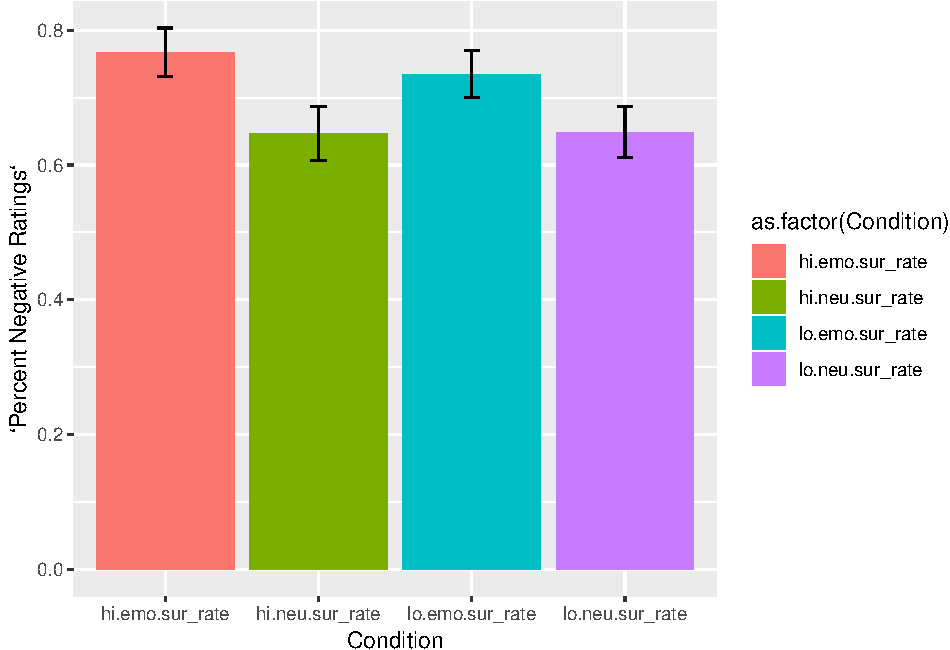
\includegraphics{Manuscript_files/figure-latex/plot figure 1-1.pdf}

Next, we assessed differences in maximum absolute deviation (MD) across the working memory trial conditions. While one of the conditions, low emotional MD, was not normally distributed (p = .024), all other conditions were normally distributed and repeated-measures ANOVA was used to analyze the MDs across conditions. There was a significant effect of load, F(1.00,196.00) = 5.51, p = .020, such that MDs under high load were larger than trials with low load. There was no significant effect of domain on MDs, F(1.00 196.00) = 0.01, p = .912, nor an interaction of load by domain, F(1.00 196.00) = 0.00, p = .960.
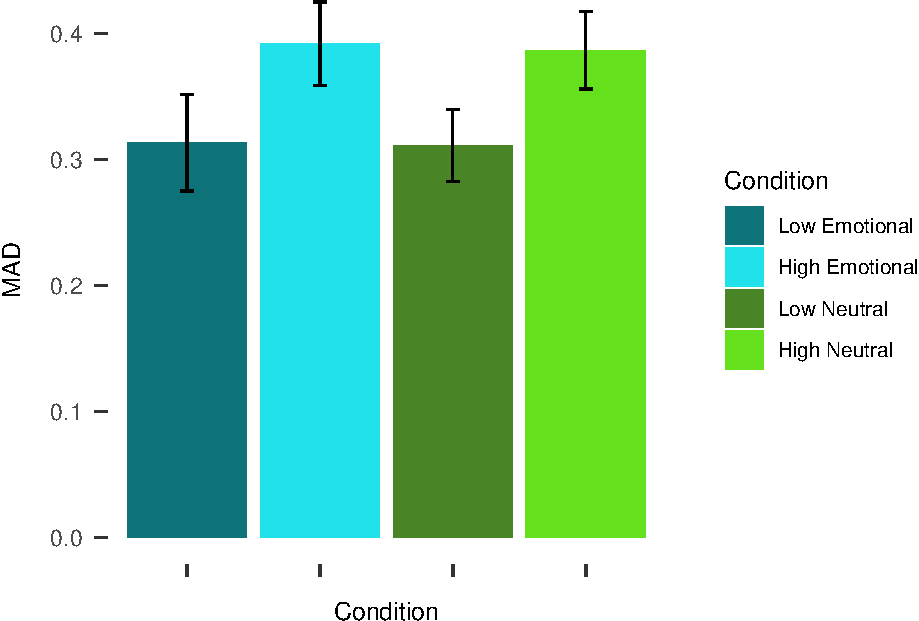
\includegraphics{Manuscript_files/figure-latex/MAD plot-1.pdf}

\hypertarget{discussion}{%
\section{Discussion}\label{discussion}}

The effect of high vs.~low load is still not apparent in these data, just like Mattek et al.~2016. An alternative explanation is that the high load manipulation is not sufficiently difficult to recruit the targeted cognitive resources; however, future work will be needed to better test this alternative.

Increased working memory demands (i.e., a higher cognitive load) do not always result in poorer performance on concurrent tasks. For instance Baddeley -(Baddeley, 1986) reported that increasing load by adding digits to a rehearsed number did not affect accuracy on a concurrent verbal reasoning task--instead, there was an increase in the latency of response, a potential interference effect that did not alter overall accuracy.

Previous work has shown that more positive interpretations of surprised faces are related to slower RTs. Our working hypothesis suggests that this delayed reaction is a result of deliberation and slower, top-down cognitive processing. It is interesting to note that, at least in these data, there is no such difference observed between the neutral and emotional WM trials, \emph{even though} the emotional WM trials are overall more negative. Future work should tease apart why this may be. For instance, \ldots{}

Future work should consider whether the representations of these emotional images in AWM (Reuter-Lorenz), or

\newpage

\hypertarget{references}{%
\section{References}\label{references}}

\begingroup
\setlength{\parindent}{-0.5in}
\setlength{\leftskip}{0.5in}

\hypertarget{refs}{}
\leavevmode\hypertarget{ref-baddeley_working_1986}{}%
Baddeley, A. D. (1986). Working memory. \emph{Philosophical Transactions of the Royal Society of London}, \emph{302}(110), 311--324.

\leavevmode\hypertarget{ref-brown_cortisol_2017}{}%
Brown, C. C., Raio, C. M., \& Neta, M. (2017). Cortisol responses enhance negative valence perception for ambiguous facial expressions. \emph{Scientific Reports}, \emph{7}(1), 15107. doi:\href{https://doi.org/10.1038/s41598-017-14846-3}{10.1038/s41598-017-14846-3}

\leavevmode\hypertarget{ref-burnham_components_2014}{}%
Burnham, B. R., Sabia, M., \& Langan, C. (2014). Components of working memory and visual selective attention. \emph{Journal of Experimental Psychology. Human Perception and Performance}, \emph{40}(1), 391--403. doi:\href{https://doi.org/10.1037/a0033753}{10.1037/a0033753}

\leavevmode\hypertarget{ref-egner_dissociable_2008}{}%
Egner, T., Etkin, A., Gale, S., \& Hirsch, J. (2008). Dissociable neural systems resolve conflict from emotional versus nonemotional distracters. \emph{Cerebral Cortex (New York, N.Y.: 1991)}, \emph{18}(6), 1475--1484. doi:\href{https://doi.org/10.1093/cercor/bhm179}{10.1093/cercor/bhm179}

\leavevmode\hypertarget{ref-freeman_mousetracker:_2010}{}%
Freeman, J. B., \& Ambady, N. (2010). MouseTracker: Software for studying real-time mental processing using a computer mouse-tracking method. \emph{Behavior Research Methods}, \emph{42}(1), 226--241. doi:\href{https://doi.org/10.3758/BRM.42.1.226}{10.3758/BRM.42.1.226}

\leavevmode\hypertarget{ref-gerin_role_2006}{}%
Gerin, W., Davidson, K. W., Christenfeld, N. J. S., Goyal, T., \& Schwartz, J. E. (2006). The role of angry rumination and distraction in blood pressure recovery from emotional arousal. \emph{Psychosomatic Medicine}, \emph{68}(1), 64--72. doi:\href{https://doi.org/10.1097/01.psy.0000195747.12404.aa}{10.1097/01.psy.0000195747.12404.aa}

\leavevmode\hypertarget{ref-hodsoll_attentional_2011}{}%
Hodsoll, S., Viding, E., \& Lavie, N. (2011). Attentional capture by irrelevant emotional distractor faces. \emph{Emotion}, \emph{11}(2), 346--353. doi:\href{https://doi.org/10.1037/a0022771}{10.1037/a0022771}

\leavevmode\hypertarget{ref-hofmann_executive_2012}{}%
Hofmann, W., Schmeichel, B. J., \& Baddeley, A. D. (2012). Executive functions and self-regulation. \emph{Trends in Cognitive Sciences}, \emph{16}(3), 174--180. doi:\href{https://doi.org/10.1016/j.tics.2012.01.006}{10.1016/j.tics.2012.01.006}

\leavevmode\hypertarget{ref-kensinger_effect_2003}{}%
Kensinger, E. A., \& Corkin, S. (2003). Effect of negative emotional content on working memory and long-term memory. \emph{Emotion}, 378--393.

\leavevmode\hypertarget{ref-lang_international_2008}{}%
Lang, P., Bradley, M. M., \& Cuthbert, B. N. (2008). International affective picture system (IAPS): Affective ratings of pictures and instruction manual., Technical Report A--8. University of Florida, Gainesville, FL.

\leavevmode\hypertarget{ref-lavie_load_2004}{}%
Lavie, N., Hirst, A., Fockert, J. W. de, \& Viding, E. (2004). Load theory of selective attention and cognitive control. \emph{Journal of Experimental Psychology: General}, \emph{133}(3), 339--354. doi:\href{https://doi.org/10.1037/0096-3445.133.3.339}{10.1037/0096-3445.133.3.339}

\leavevmode\hypertarget{ref-lundqvist_karolinska_1998}{}%
Lundqvist, D., Flykt, A., \& Öhman, A. (1998). The karolinska directed emotional faces---KDEF (CD ROM)., Stockholm: Karolinska Institute, Departmentof Clinical Neuroscience, PsychologySection.

\leavevmode\hypertarget{ref-mathews_cognitive_2005}{}%
Mathews, A., \& MacLeod, C. (2005). Cognitive vulnerability to emotional disorders. \emph{Annual Review of Clinical Psychology}, \emph{1}, 167--195. doi:\href{https://doi.org/10.1146/annurev.clinpsy.1.102803.143916}{10.1146/annurev.clinpsy.1.102803.143916}

\leavevmode\hypertarget{ref-mattek_differential_2016}{}%
Mattek, A. M., Whalen, P. J., Berkowitz, J. L., \& Freeman, J. B. (2016). Differential effects of cognitive load on subjective versus motor responses to ambiguously valenced facial expressions. \emph{Emotion}, \emph{16}(6), 929--936. doi:\href{https://doi.org/10.1037/emo0000148}{10.1037/emo0000148}

\leavevmode\hypertarget{ref-neta_through_2018}{}%
Neta, M., \& Dodd, M. D. (2018). Through the eyes of the beholder: Simulated eye-movement experience (``SEE'') modulates valence bias in response to emotional ambiguity. \emph{Emotion}, \emph{18}(8), 1122--1127. doi:\href{https://doi.org/10.1037/emo0000421}{10.1037/emo0000421}

\leavevmode\hypertarget{ref-neta_neural_2013}{}%
Neta, M., Kelley, W. M., \& Whalen, P. J. (2013). Neural responses to ambiguity involve domain-general and domain-specific emotion processing systems. \emph{Journal of Cognitive Neuroscience}, \emph{25}(4), 547--557. doi:\href{https://doi.org/10.1162/jocn_a_00363}{10.1162/jocn\_a\_00363}

\leavevmode\hypertarget{ref-neta_corrugator_2009}{}%
Neta, M., Norris, C. J., \& Whalen, P. J. (2009). Corrugator muscle responses are associated with individual differences in positivity-negativity bias. \emph{Emotion (Washington, D.C.)}, \emph{9}(5), 640--648. doi:\href{https://doi.org/10.1037/a0016819}{10.1037/a0016819}

\leavevmode\hypertarget{ref-neta_dont_2016}{}%
Neta, M., \& Tong, T. T. (2016). Don't like what you see? Give it time: Longer reaction times associated with increased positive affect. \emph{Emotion (Washington, D.C.)}, \emph{16}(5), 730--739. doi:\href{https://doi.org/10.1037/emo0000181}{10.1037/emo0000181}

\leavevmode\hypertarget{ref-neta_its_2018}{}%
Neta, M., Tong, T. T., \& Henley, D. J. (2018). It's a matter of time (perspectives): Shifting valence responses to emotional ambiguity. \emph{Motivation and Emotion}, \emph{42}, 258--266. doi:\href{https://doi.org/10.1007/s11031-018-9665-7}{10.1007/s11031-018-9665-7}

\leavevmode\hypertarget{ref-neta_all_2017}{}%
Neta, M., Tong, T. T., Rosen, M. L., Enersen, A., Kim, M. J., \& Dodd, M. D. (2017). All in the first glance: First fixation predicts individual differences in valence bias. \emph{Cognition \& Emotion}, \emph{31}(4), 772--780. doi:\href{https://doi.org/10.1080/02699931.2016.1152231}{10.1080/02699931.2016.1152231}

\leavevmode\hypertarget{ref-neta_primacy_2010}{}%
Neta, M., \& Whalen, P. J. (2010). The primacy of negative interpretations when resolving the valence of ambiguous facial expressions. \emph{Psychological Science}, \emph{21}(7), 901--907. doi:\href{https://doi.org/10.1177/0956797610373934}{10.1177/0956797610373934}

\leavevmode\hypertarget{ref-petro_individual_2018}{}%
Petro, N. M., Tong, T. T., Henley, D. J., \& Neta, M. (2018). Individual differences in valence bias: fMRI evidence of the initial negativity hypothesis. \emph{Social Cognitive and Affective Neuroscience}, \emph{13}(7), 687--698. doi:\href{https://doi.org/10.1093/scan/nsy049}{10.1093/scan/nsy049}

\leavevmode\hypertarget{ref-piech_attentional_2011}{}%
Piech, R. M., McHugo, M., Smith, S. D., Dukic, M. S., Van Der Meer, J., Abou-Khalil, B., \ldots{} Zald, D. H. (2011). Attentional capture by emotional stimuli is preserved in patients with amygdala lesions. \emph{Neuropsychologia}, \emph{49}(12), 3314--3319. doi:\href{https://doi.org/10.1016/j.neuropsychologia.2011.08.004}{10.1016/j.neuropsychologia.2011.08.004}

\leavevmode\hypertarget{ref-schmeichel_working_2008}{}%
Schmeichel, B. J., Volokhov, R. N., \& Demaree, H. A. (2008). Working memory capacity and the self-regulation of emotional expression and experience. \emph{Journal of Personality and Social Psychology}, \emph{95}(6), 1526--1540. doi:\href{https://doi.org/10.1037/a0013345}{10.1037/a0013345}

\leavevmode\hypertarget{ref-shaw_dieting_2004}{}%
Shaw, J., \& Tiggemann, M. (2004). Dieting and working memory: Preoccupying cognitions and the role of the articulatory control process. \emph{British Journal of Health Psychology}, \emph{9}(Pt 2), 175--185. doi:\href{https://doi.org/10.1348/135910704773891032}{10.1348/135910704773891032}

\leavevmode\hypertarget{ref-stroop_studies_1935}{}%
Stroop, J. R. (1935). Studies of interference in serial verbal reactions. \emph{Journal of Experimental Psychology}, \emph{18}(6), 643--662. doi:\href{https://doi.org/10.1037/h0054651}{10.1037/h0054651}

\leavevmode\hypertarget{ref-tottenham_nimstim_2009}{}%
Tottenham, N., Tanaka, J. W., Leon, A. C., McCarry, T., Nurse, M., Hare, T. A., \ldots{} Nelson, C. (2009). The NimStim set of facial expressions: Judgments from untrained research participants. \emph{Psychiatry Research}, \emph{168}(3), 242--249. doi:\href{https://doi.org/10.1016/j.psychres.2008.05.006}{10.1016/j.psychres.2008.05.006}

\leavevmode\hypertarget{ref-van_dillen_tuning_2009}{}%
Van Dillen, L. F., Heslenfeld, D. J., \& Koole, S. L. (2009). Tuning down the emotional brain: An fMRI study of the effects of cognitive load on the processing of affective images. \emph{NeuroImage}, \emph{45}(4), 1212--1219. doi:\href{https://doi.org/10.1016/j.neuroimage.2009.01.016}{10.1016/j.neuroimage.2009.01.016}

\leavevmode\hypertarget{ref-whalen_emotional_2006}{}%
Whalen, P. J., Bush, G., Shin, L. M., \& Rauch, S. L. (2006). The emotional counting stroop: A task for assessing emotional interference during brain imaging. \emph{Nature Protocols}, \emph{1}(1), 293--296. doi:\href{https://doi.org/10.1038/nprot.2006.45}{10.1038/nprot.2006.45}

\leavevmode\hypertarget{ref-yang_positive_2013}{}%
Yang, H., Yang, S., \& Isen, A. M. (2013). Positive affect improves working memory: Implications for controlled cognitive processing. \emph{Cognition and Emotion}, \emph{27}(3), 474--482. doi:\href{https://doi.org/10.1080/02699931.2012.713325}{10.1080/02699931.2012.713325}

\endgroup


\end{document}
